%GD can be used in many scenarios such as multi-task learning, semi-supervised learning, and reinforcement learning. 
As generalized distillation only requires the training inputs $\{x_i,y_i\}_{i=1}^n$ and the output $s_i$ from the teacher function $f^{(t)}$ when training, it can be naturally applied to SDA. This leads to \textit{Generalized Distillation Semi-supervised Domain Adaptation} (\textbf{GDSDA}), where the source model can be used as the teacher to output the soft labels and the student model is the target model. Moreover, in GDSDA, we also consider the multi-source scenario and extend the GD paradigm to fit this scenario. To be consistent with other work in domain adaptation, we use source model and target model to denote the teacher model and the student model in the rest of our paper in GDSDA.

An important issue of applying GD to SDA is that, in Eq. \eqref{eq:distill}, each example is assigned with a hard label $y$ (true label) and a soft label $s$ (class probabilities from the teacher). However, in SDA, we are not able to obtain the hard labels of the unlabeled data. Here we follow \cite{lopez2015unifying} and use the "fake label" strategy to label the unlabeled data: for the labeled examples, we use \textit{one-hot} strategy to encode their labels while using 0s as the labels of the unlabeled examples. Thus, each example in the target domain is assigned with a label. It is arguable that the "fake label" strategy would introduce extra noise and degrade the performance. However, we will show in our experiment that this noise can be well controlled by setting a proper value to the imitation parameter and we can still achieve improved performance (See the single source experiment).
\begin{figure}
	\centering
	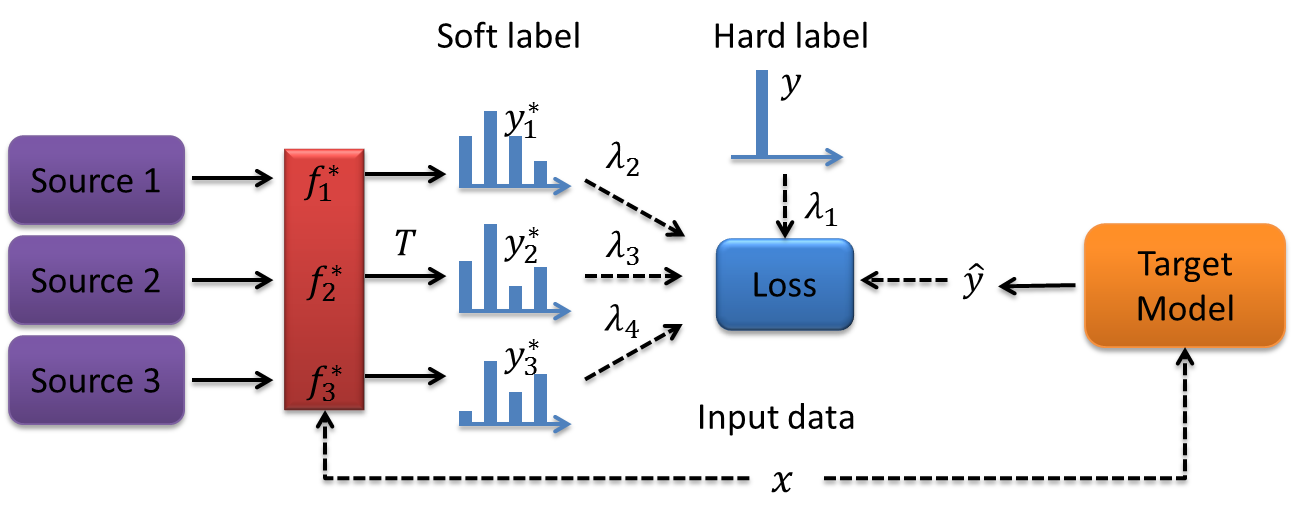
\includegraphics[scale=.4]{figure/multi-GDDA.png}
	\caption{Illustration of GDSDA training process.}
	\label{fig:GDSDA}
\end{figure}
 
The process of GDSDA is shown in Figure \ref{fig:GDSDA}. Suppose we have $M-1$ source domains denoted as $D_s^{(j)}=\{X^{(j)},Y^{(j)}\}_{j=1}^{M-1}$ and the target domain $D_t=\{X,Y\}$ encoded with the "fake label" strategy. The process of GDSDA is as follows:
\begin{enumerate}
    \item Train the source models $f^*_j$ for each of the $M-1$ domains with $\{X^{(j)},Y^{(j)}\}$.
    \item For each of the training example $x_i$ in the target domain, computer the corresponding soft label $y^*_{ij}$ with each of the source model $f^*_j$ and the temperature $T>0$.
    \item Learn the target model $f_t$ using the $(M+1)$-tuples $\{x_i,y_i,y^*_{i1},\dots,y^*_{i(M-1)}\}_{i=1}^L$ with the imitation parameters $\{\lambda_i\}^M_{i=1}$ using \eqref{eq:GDDA_abs}:
\end{enumerate} 
\begin{equation}\label{eq:GDDA_abs}
\begin{aligned}
f_t(\lambda)=\underset{f_t \in \mathcal{F}}{\arg \min}&\frac{1}{L}\sum_{i=1}^{L}\bigg[\lambda_1\ell\left(y_i,f_t(x_i)\right)+\sum_{j=1}^{M-1}\lambda_{j+1}\ell\left(y^*_{ij},f_t(x_i)\right)\bigg]\qquad\\
 &\text{s.t.} \qquad \sum_i\lambda_i=1
\end{aligned}
\end{equation}
Compared to other work of SDA which requires to use each example of the source domain, by either re-weighting \cite{Donahue_2013_CVPR,duan2012visual} or feature augmentation \cite{daume2010frustratingly}, GDSDA only requires the trained model from the source domain to generate the soft labels. 
%Considering the fact that it is more convenient to access the source model than each of the examples of the source domain, GDSDA can be more useful than those previous methods. For example, if we want to use ImageNet \cite{imagenet_cvpr09} as the source domain, it is almost impossible to access each of the millions of the examples while there are many well trained models publicly available online that can be used for GDSDA. 
Meanwhile, GDSDA is able to handle the multi-class scenario while some previous work, such as SHFA\cite{duan2012learning} can only solve the binary classification problem in SDA. Moreover, GDSDA is able to transfer the knowledge from any type of source model that is able to output the soft label (class probabilities) without accessing the source data.

\subsection{Why does GDSDA work}
In this part, we demonstrate the scenarios where GDSDA would work. Before we provide our analysis, we first introduce the two basic assumptions of GDSDA: the \textit{assumption of distillation} and \textit{the assumption of the source model}.

\textbf{Assumption of distillation:} The capacity (VC dimension) of the target model $f_t$ is smaller than the capacity of source model $f^*$. This assumption is inherited from GD.
\textbf{Assumption of the source model:} The source model $f^*$ should work better than a target model $f'_t$ trained only with the hard labels. 
This assumption is based on a simple fact that it is more effective to learn from a superior model. This assumption is very common especially in SDA where the labeled data is often too few to build a good target model alone.
For example, when we only have a single labeled example for each class in the target training set, it is reasonable to assume that the source model trained from another domain could perform better than any model trained only with the target training data on the target task. %Based on this two assumptions, we will show that GDSDA can effectively leverage the source model and transfer the knowledge between different domains under the SDA setting.

Suppose the complex source model $f^*$ can generalize well on target domain. The simple target model $f_t$ generalizes the same way as the source model $f^*$ would typically do better than the source model $f^*$ itself as well as the target model trained only with hard labels on the target domain (according to the assumption of the source model). This means the knowledge can be transferred smoothly between models. Specifically, as it is suggested in \cite{hinton2015distilling}, the transfer process can be achieved by letting the target model mimick the outputs of the source model (soft labels) on the training set without considering the true labels of the training examples. In another word, the useful source knowledge can be effectively transferred with the unlabeled data.

As the source models is trained from the source domains, it is reasonable to weigh the source knowledge due to the domain shift\cite{karl2001long} when we apply it to the target domain. In Eq. \eqref{eq:GDDA_abs}, we use the hyperparameter $\lambda$, called imitation parameter, to control the relative importance between the soft labels and the hard labels, which in turn reflects the amount of the knowledge transferred from each of the source models. Specifically, the larger value of the imitation parameter is, the more important the soft labels are and more knowledge is transferred from the source domains. 
For example, in Figure \ref{fig:GDSDA}, when we set $\lambda_2=0$, we actually ignore the knowledge from source domain 1.
As a result, with the proper imitation parameter, GDSDA can effectively transfer the knowledge from each of the source models under the setting of SDA (for more details, please see the experiment section).

How to choose the imitation parameter is essential for GDSDA.
Many previous studies have addressed the importance of knowledge transfer control in domain adaptation\cite{duan2012learning,duan2012visual}. Without carefully controlling the amount of knowledge transferred from the source domain, it is easy for the target model to get degraded performance or even suffer from negative transfer\cite{pan2010survey}. However, in the previous studies, the imitation parameter can only be determined by either brute force search\cite{lopez2015unifying} or background knowledge\cite{Tzeng_2015_ICCV} which scale poorly with the number of available source model and imitation parameter.
Therefore, we propose our method, called GDSDA-SVM that can estimate the transfer parameter automatically.

%In the following, we show that we should choose the imitation parameter that minimizes the empirical risk on the training data for distillation.

%Let $f(x,\lambda)$ be a function with a finite VC dimension $h$ that minimizes the number of errors on the training data $\{x_i,y_i\}_{i=1}^L$. Let $v(\lambda)$ be the training error. Then according to the VC theory \cite{vapnik1999overview}, for an arbitrary loss function $\mathcal{L}(\cdot)$ we have the following bound:
%\begin{equation}\label{eq:lambda_constraint}
%P\left(\mathcal{L}\left(y,f(x,\lambda)\right)\geq 0\right) < v(\lambda)+O\left(\sqrt{\frac{h}{L}}\right)
%\end{equation}
%In other word, the optimal imitation parameter should be the one that can minimize the training error.  

%In the previous work, the imitation parameter can only be determined by either brute force search \cite{lopez2015unifying} or background knowledge \cite{Tzeng_2015_ICCV} which greatly reduces its effectiveness. In domain adaptation, it is common that there could be multiple source models to be exploited. It is ideal to find a method that can determine the imitation parameter automatically.
